
%
% raspberry p3 spec: https://www.raspberrypi.org/magpi/raspberry-pi-3-specs-benchmarks/

\section{Embedded Computing Platform Comparison}\label{sec:comparison}

%% \begin{figure}[h]
%%   \centering
%%   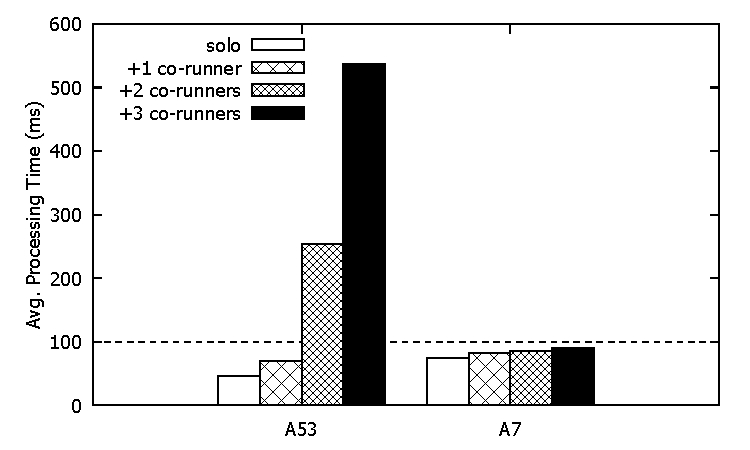
\includegraphics[width=.45\textwidth]{figs/a53_vs_a7}
%%   \caption{DNN model performance on different in-order
%% ARM Cortex cores. \fixme{this may be better in the plaform comparison section}.}
%%   \label{fig:a53_vs_a7}
%% \end{figure}


\begin{table*}[h]
  \centering
  \begin{adjustbox}{width=1\textwidth}
  \begin{tabular}{|c|c|c|c|}
    \hline
    Item    & Raspberry Pi 3 (B)   & Intel UP                  & NVIDIA Jetson TX2\\
    \hline
            & BCM2837              & X5-Z8350 (Cherry Trail)   & Tegra X2 \\
    CPU     & 4x Cortex-A53@1.2GHz/512KB L2  &
              4x Atom@1.92GHz/2MB L2 &
              4x Cortex-A57@2.0GHz/2MB L2 \\
            &              &              & 2x Denver@2.0GHz/2MB L2 (not used)  \\
    \hline
    GPU     &  VideoCore IV (not used)    &
               Intel HD 400 Graphics (not used) &
               Pascal 256 CUDA cores   \\
    \hline
    Memory  & 1GB LPDDR2   &  2GB DDR3L     & 8GB LPDDR4              \\
    \hline
	Peak Memory Bandwidth & 8.5 GB/s & 12.8 GB/s & 59.7 GB/s \\
	%% \hline
	%% Measured Bandwidth & 2127.94 MB/s & 3951.94 MB/s & 4447.90 MB/s \\
	\hline
	Cost  & \$35 & \$100 & \$600 \\
	\hline
  \end{tabular}
  \end{adjustbox}
  \caption{Compared embedded computing platforms}
  \label{tbl:platforms}
\end{table*}

In this section, we compare three computing platforms---the Raspberry
Pi 3, the Intel UP~\cite{intelup} and the NVIDIA Jetson
TX2~\cite{nvidiajetson}---from the point of view of supporting
end-to-end deep learning based autonomous vehicles. 
Table~\ref{tbl:platforms} shows the architectural features of the three
platforms~\footnote{The GPU of Intel UP and the two Denver cores in the
  Tegra TX2 are not used in evaluation due to TensorFlow issues.}.
  
Our basic approach is to use the same DeepPicar software, and repeat
the experiments in Section~\ref{sec:evaluation} on each hardware
platform and compare the results. 
%We do not, however, repeat the cache
%partitioned experiments done on the Pi 3, as we did not believe our 
%findings warranted further experimentation on additional platforms. 
For the Jetson TX2, we have two different system configurations,
which differ in whether TensorFlow is configured to use its GPU or
only the CPU cores. Thus, a total of four system configurations are
compared.

\begin{figure}[h]
  \centering
  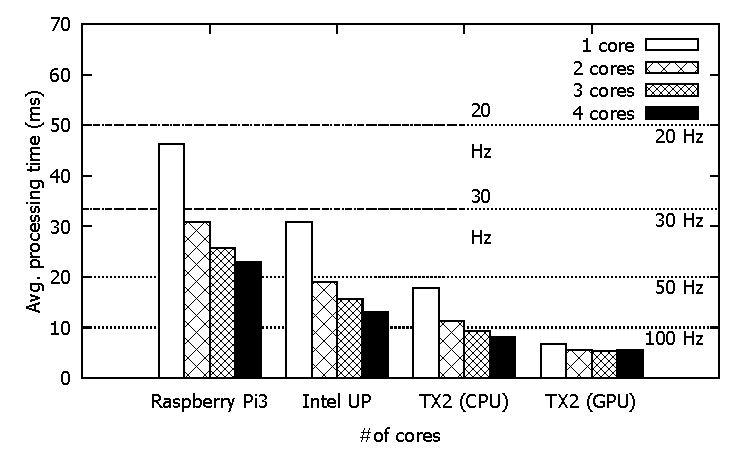
\includegraphics[width=.45\textwidth]{figs/compare_core}
  \caption{Average control loop execution time.} 
  \label{fig:sys_core}
\end{figure}

Figure~\ref{fig:sys_core} shows the average control loop completion
timing of the four system configurations we tested as a function of
the number of CPU cores used. (cf. Figure~\ref{fig:perf-vs-corecnt})
Both the Intel UP and Jetson TX2 exhibit better performance than
Raspberry Pi 3. When all four CPU cores are used, the Intel UP is
1.33X faster than Pi 3, while the TX2 (CPU) and TX2 (GPU) are 2.79X and
4.16X times faster that the Pi 3, respectively.
Thus, they all satisfy 33.3 ms WCET by a clear margin, and, in the
case of the TX2, 50 Hz or even 100 Hz real-time control is feasible
with the help of its GPU.
Another observation is that the CNN task's performance on TX2 (GPU)
does not change much as we increase the number of cores. This
is because most of the neural network computation is done by the GPU.

\begin{figure}[h]
  \centering
  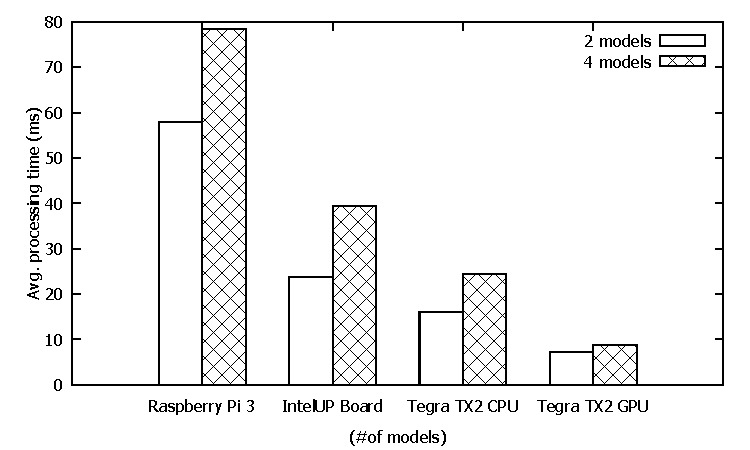
\includegraphics[width=.45\textwidth]{figs/compare_model}
  \caption{Timing impact of co-scheduling multiple CNNs on different
    embedded multicore platforms. %% 1Nx1C: one DNN
    %% model using one core; 4Nx1C: four DNN models each using one core;
    %% 1Nx2C: one DNN model using two cores; 2Nx2C: two DNN models each
    %% using two cores.
  }
  \label{fig:sys_model}
\end{figure}

Figure~\ref{fig:sys_model} shows the results of the
multi-model co-scheduling experiment
(cf. Figure~\ref{fig:perf-vs-modelcnt}). Once again, they can comfortably
satisfy 30 Hz real-time performance for all of the co-scheduled CNN control
loops, and in the case of the TX2 (GPU), even 100 Hz real-time control
is feasible in all co-scheduling setups.
Given that the GPU must be shared among the co-scheduled CNN
models, the results suggest that the TX2's GPU has sufficient capacity to
accomodate multiple instances of the CNN models we tested.

\begin{figure}[h]
  \centering
  \begin{subfigure}{0.45\textwidth}
    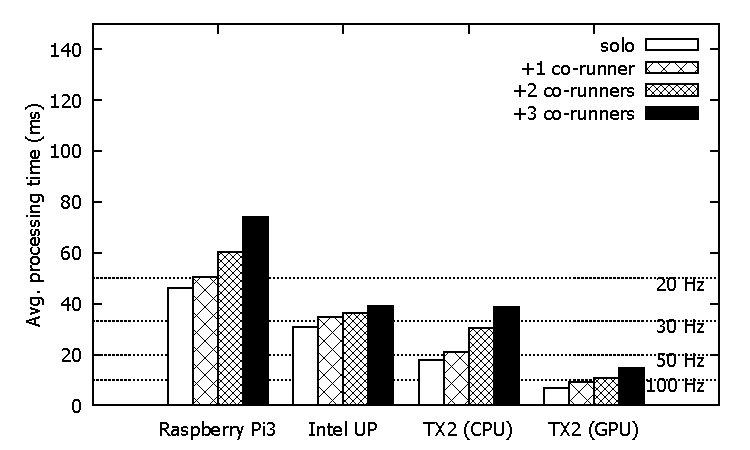
\includegraphics[width=\textwidth]{figs/compare_benchmark_read}
    \caption{BwRead}
    \label{fig:sys_bench_read}
  \end{subfigure}
  \hfill
  \begin{subfigure}{0.45\textwidth}
    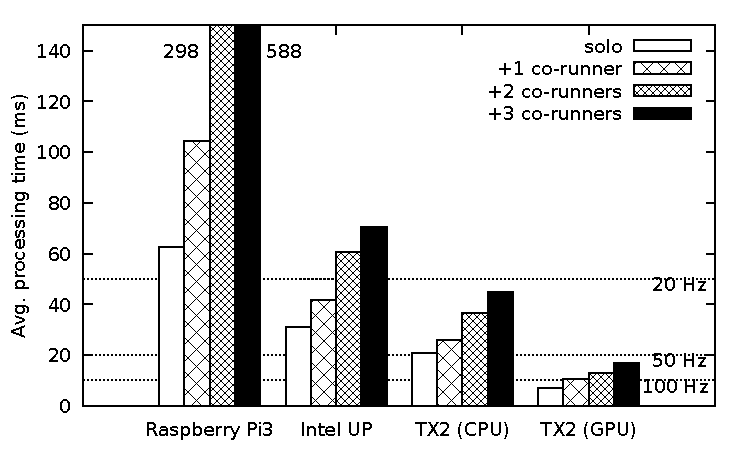
\includegraphics[width=\textwidth]{figs/compare_benchmark}
    \caption{BwWrite}
    \label{fig:sys_bench_write}    
  \end{subfigure}
  \caption{Average processing time vs. the number of memory
    intensive co-runners.}
  \label{fig:sys_bench}    
\end{figure} 

Figure~\ref{fig:sys_bench} shows the results of the synthetic memory
intensive task co-scheduling experiments
(cf. Figure~\ref{fig:perf_vs_bandwidth}).
For read co-runners (BwRead), the performance of all platforms
gradually decreased as additional BwRead instances were introduced: up
to 1.6X for the Pi 3, up to 1.3X for the Intel UP, and up to 1.6X and 2.2X for
the TX2 (CPU) and TX2(GPU), respectively.
For write co-runners (BwWrite), however, we observe generally more
noticieable execution time increases. As we discussed
earlier in Section~\ref{sec:evaluation}, the Pi 3 suffers up to 11.6X
execution time increase, while the Intel UP and Jetson TX2 suffer less
dramatic but still significant execution time increases.

%% Compared to their respective solo timings  
%% (i.e., the model runs on a single core in isolation), Intel UP suffers up to
%% 2.3X execution time increase; TX2 (CPU) and TX2 (GPU) both suffer up to
%% 2.3X increases. This is somewhat surprising
%% because the Raspberry Pi 3's cores are in-order architecture based while
%% the cores in the Intel Up and NVIDIA TX2 are out-of-order architecture
%% based, and that the memory intensive tasks on out-of-order cores can
%% generate more memory traffic.
%% We believe that this is because the
%% memory subsystems in the Intel UP and TX2 platforms provide higher
%% performance than the memory subsystem of the Pi 3 as suggested from
%% the measured memory bandwidth results in Table~\ref{tbl:platforms}
%% ('Measured Bandwidth').

Another interesting observation is that the TX2 (GPU) also suffers
considerable execution time increase (2.3X) despite the fact that the
co-scheduled synthetic tasks do not utilize the GPU (i.e., the CNN
model has dedicated access to the GPU.) This is, however, a 
known characteristic of integrated CPU-GPU architecture based
platforms in which both the CPU and GPU share the same memory
subsystem~\cite{Ali2017} and therefore can suffer bandwidth contention
as we observe in this case.

%% \begin{figure}[h]
%%   \centering
%%   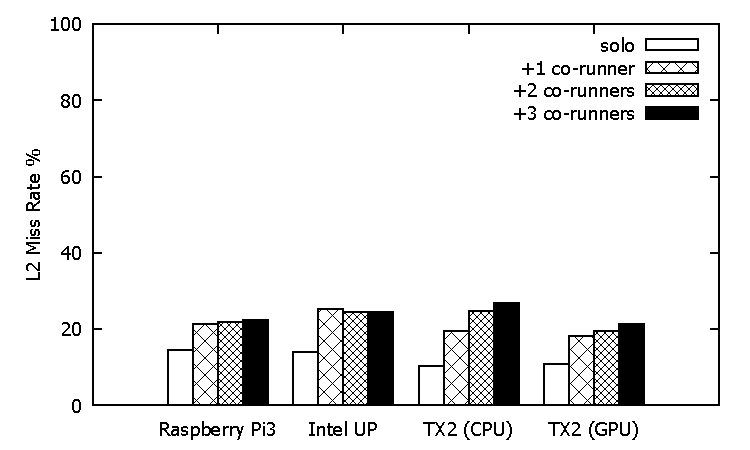
\includegraphics[width=.45\textwidth]{figs/compare_readl2}
%%   \caption{L2 miss rates in the presence of an increasing number of 
%% 			memory intensive read applications on idle CPU cores.}
%%   \label{fig:sys_readl2miss}
%% \end{figure}

%% \begin{figure}[h]
%%   \centering
%%   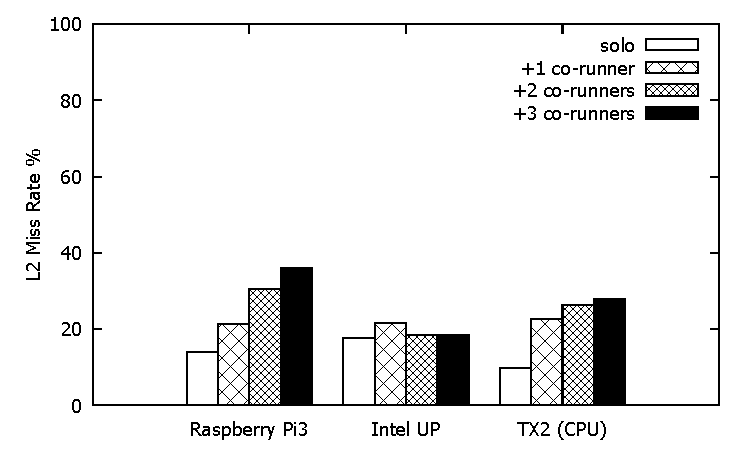
\includegraphics[width=.45\textwidth]{figs/compare_l2missrate}
%%   \caption{L2 miss rates in the presence of an increasing number of 
%% 			memory intensive write applications on idle CPU cores.}
%%   \label{fig:sys_l2miss}
%% \end{figure}

%% Figures~\ref{fig:sys_readl2miss} and ~\ref{fig:sys_l2miss} show
%% the L2 miss rates of DNN control loops when read and write co-runners
%% are introduced, respectively. The key takeaway of this result is that the 
%% L2 miss rate is a
%% poor indicator to the execution time of the control loop. As shown
%% already, the Raspberry Pi 3's increased L2 misses do not fully explain
%% increases in processing times. In case of the Intel UP, as the number of
%% interfering Bandwidth benchmark instances increases, the L2 miss rates
%% drop slightly. In the case of the TX2 (CPU), from solo to one co-runner,
%% L2 miss rates almost double, but then the execution time
%% increase is a little less than 10\%. However, when there are
%% co-runners, even though the L2 miss rates are largely unchanged, the
%% CNN processing time increases significantly. The TX2 (GPU) also shows
%% similar behavior. All of these results essentially point to the fact
%% that DNN inferencing workload is largely memory performance sensitive
%% but not L2 cache space sensitive. 

%% \begin{figure}[h]
%%   \centering
%%   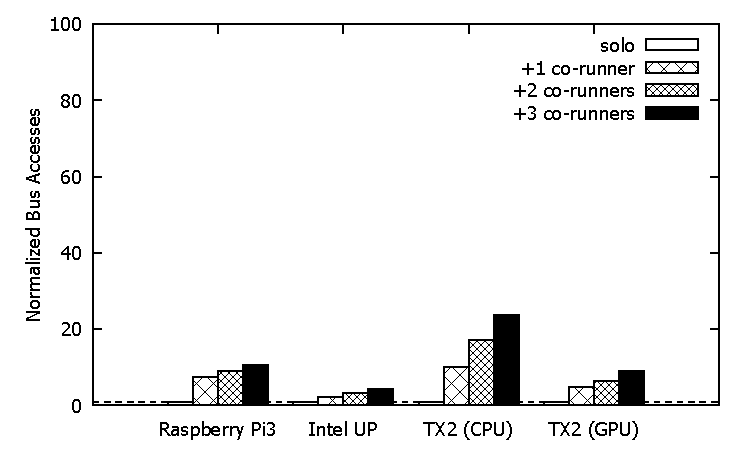
\includegraphics[width=.45\textwidth]{figs/compare_readbus}
%%   \caption{Bus accesses in the presence of an increasing number of 
%% 			memory intensive read applications on idle CPU cores.}
%%   \label{fig:sys_readbus}
%% \end{figure}

%% \begin{figure}[h]
%%   \centering
%%   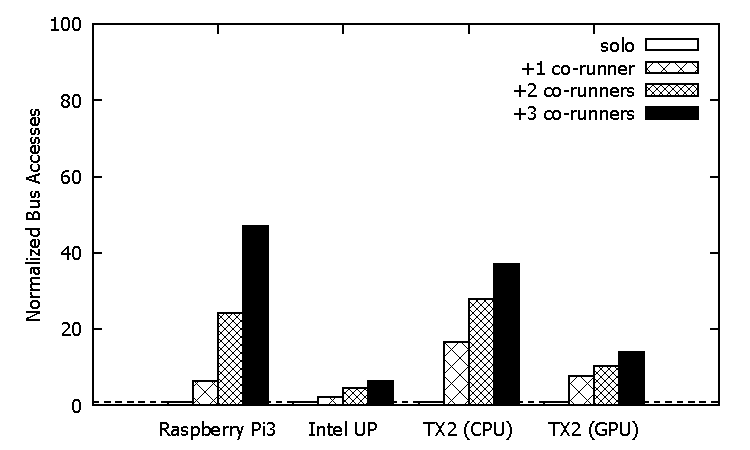
\includegraphics[width=.45\textwidth]{figs/compare_writebus}
%%   \caption{Bus accesses in the presence of an increasing number of 
%% 			memory intensive write applications on idle CPU cores.}
%%   \label{fig:sys_writebus}
%% \end{figure}

%% \color{red}FIXME: I believe the bus access results for the Intel UP are wrong. 
%% I couldn't get the IDI off-core response event to work, so I used the bus-cycles 
%% perf event, which I think is incorrect.

%% \color{black}Figures~\ref{fig:sys_readbus} and ~\ref{fig:sys_writebus} show the
%% normalized bus accesses for each of the platforms as read and write
%% co-runners are introduced, respectively. Unlike the L2 miss rates of the
%% model, the total number of bus accesses more closely align with the 
%% execution time increases that are seen in each of the platforms. For the Pi 3, both 
%% the execution time and bus accesses increase at exponential rates. In the TX2(GPU), 
%% the bus accesses increase in a similar linear fashion to the execution time. The main outlier
%% is the TX2(CPU) which has bus accesses increase at a faster rate similar to that of the Pi 3.
%% However, the bus accesses seem to increase linearly, which is also seen in the
%% execution time. As a result, we find that the total number of bus accesses have a higher 
%% correlation to the model execution time than L2 miss rates.

%% %% However, the L2 miss rates of the Pi 3 and TX2 platforms follow the same expected 
%% %% pattern, as can be seen in Figure~\ref{fig:sys_l2miss}. Namely, the 
%% %% percentage of L2 miss rates increases are more 
%% %% memory intensive co-runners are introduced. This was not the case for 
%% %% the UP board, where the model running on two cores generated the highest
%% %% percentage of L2 cache misses. This is most likely due to the CPU 
%% %% architecture of the UP's CPU which is Intel based, whereas both the Pi 3
%% %% and TX2 have ARM based CPUs.


In summary, we find that todays embedded computing platforms, even as
inexpensive as a Raspberry Pi 3, are powerful enough to support
CNN based real-time control applications. Furthermore, availability of
CPU cores and a GPU on these platforms allows consolidating multiple CNN
workloads. However, shared resource contention among these diverse
computing resources remains an important issue that must be understood
and controlled, especially for safety-critical applications.
